\chapter{Evaluation Results}
\label{cha:evaluationResults}

In this chapter we present algorithm evaluation results and conclusions.

\section{Testing rig}

All algorithms were run on Lenovo W530 notebook with the following hardware and software:
\begin{itemize}
	\item CPU: Intel Core i7-3740QM (2.7 GHz)
	\item RAM size: 16 GB
	\item Operating system: Windows 7 Enterprise 64-bit
\end{itemize}

All tests were performed under "Maximum Performance" setting.

\section{Test data}

Numerous test cases were generated, varying in problem size, number of winners, generation model and satisfaction function.

\subsection{Problem size}

Problem size is defined by number of agents ($n$) and number of alternatives ($m$). We selected three problem sizes for testing:
\begin{itemize}
	\item Small instance: $n = 30$, $m = 10$
	\item Medium instance: $n = 400$, $m = 50$
	\item Large instance: $n = 400$, $m = 300$
\end{itemize}

\subsection{Number of winners}

For each problem size, we selected two different number of winners ($K$) - first one to take a small part of alternatives as winners (around 15-20\%) and the second one to take about half of alternatives as winners:
\begin{itemize}
	\item Small instance: $K = 2$ or $K = 5$
	\item Medium instance: $K = 10$ or $K = 25$
	\item Large instance: $K = 50$ or $K = 200$
\end{itemize}

\subsection{Data generation model}

Test data was generated using two different models.
\\

\noindent
\textbf{Polya urn model} (Polya) \hspace{.1in} This model assumes we have an urn with $m$ balls in $m$ colors, each representing an alternative. We generate preferences by drawing random balls from the urn. First, we draw alternatives for first rank in each agent's preference order, then for second ranks, and so on, until the entire preference profile is drawn. After the ball is drawn, it is returned to the urn and another ball of the same color is added to the urn too, so a probability of drawing the same color in the future is increased ("strong becomes stronger"). The only constraint is that an alternative cannot be drawn for an agent for which it has been already drawn before. This model generates preference profile where some relatively small number of alternatives is preferred to all the others by most agents.
\\

\noindent
\textbf{Impartial culture model} (IC) \hspace{.1in} In this model, for each agent we generate preference order independently. For each agent, every preference order (every permutation of alternatives) has equal probability of being drawn. This model generates preference profile with no clearly dominating alternatives.

\subsection{Satisfaction function}

Two different satisfaction functions were used, each of them trying to model real preferences of the voters.
\\

\noindent
\textbf{Square function} \hspace{.1in} This is simply a square function and it assumes that difference between voters in the first positions of the preference order should be higher than between the last positions (voter is more concerned with his favourite candidates, not the ones at the end of the list). The function is given as follows:

\begin{gather}
	\alpha(i) = (m - i)^{2}
\end{gather}
\\

Example of function for $m = 20$:

\begin{center}
	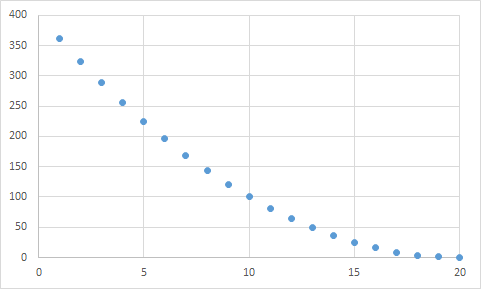
\includegraphics[scale=0.75]{satfun1}
\end{center}

\noindent
\textbf{Strange function} \hspace{.1in} This function assumes that for the voter the difference between two candidates from the top is the same as the difference between two candidates from the bottom, while differences between candidates from the middle of the preference order are much less significant. The function is given as follows:

\begin{gather}
	f(x) = \frac{x^{2}+x}{2} \\
	h = \frac{m}{2} \\
	d = f(h) \\
	\alpha(i) = \begin{cases} f(h-i+1)+d-1 : i<h \\ -f(i-h)+d : i \geq h \end{cases}
\end{gather}
\\

Example of function for $m = 20$:

\begin{center}
	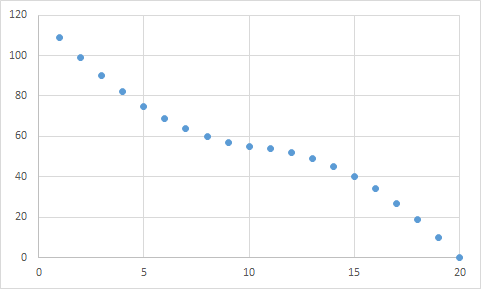
\includegraphics[scale=0.75]{satfun2}
\end{center}

\subsection{Summary}

Table below presents all generated test cases.

\begin{tabular}{r | c | c | c | c | c |}
	\# & alternatives count & agents count & winners count & generation model & satisfaction function \\
	\hline
	1 & \multirow{8}{*}{10} & \multirow{8}{*}{30} & \multirow{4}{*}{2} & \multirow{2}{*}{Polya} & Square \\
	2 & & & & & Strange \\
	\cline{5-6}
	3 & & & & \multirow{2}{*}{IC} & Square \\
	4 & & & & & Strange \\
	\cline{4-6}
	5 & & & \multirow{4}{*}{5} & \multirow{2}{*}{Polya} & Square \\
	6 & & & & & Strange \\
	\cline{5-6}
	7 & & & & \multirow{2}{*}{IC} & Square \\
	8 & & & & & Strange \\
	\hline
	9 & \multirow{8}{*}{50} & \multirow{8}{*}{400} & \multirow{4}{*}{10} & \multirow{2}{*}{Polya} & Square \\
	10 & & & & & Strange \\
	\cline{5-6}
	11 & & & & \multirow{2}{*}{IC} & Square \\
	12 & & & & & Strange \\
	\cline{4-6}
	13 & & & \multirow{4}{*}{25} & \multirow{2}{*}{Polya} & Square \\
	14 & & & & & Strange \\
	\cline{5-6}
	15 & & & & \multirow{2}{*}{IC} & Square \\
	16 & & & & & Strange \\
	\hline
	17 & \multirow{8}{*}{300} & \multirow{8}{*}{400} & \multirow{4}{*}{50} & \multirow{2}{*}{Polya} & Square \\
	18 & & & & & Strange \\
	\cline{5-6}
	19 & & & & \multirow{2}{*}{IC} & Square \\
	20 & & & & & Strange \\
	\cline{4-6}
	21 & & & \multirow{4}{*}{200} & \multirow{2}{*}{Polya} & Square \\
	22 & & & & & Strange \\
	\cline{5-6}
	23 & & & & \multirow{2}{*}{IC} & Square \\
	24 & & & & & Strange \\
	\hline
\end{tabular}
\\

\section{Test Methodology}

For each combination of problem size and generation model 100 files were generated independently. Algorithms were evaluated against all test files for each test case. We measured execution time and solution quality (total satisfaction) which was compared with brute-force (optimal) result for small instances and upper bound (total satisfaction if every agent has his top alternative assigned) for medium and large instances. Execution time and solution quality comparison with brute-force result or upper bound are presented as an average of 100 results (with standard deviation).
\\

All test cases were used for both Chamberlin-Courant and Monroe problems.

\section{Chamberlin-Courant Problem Evaluation}

In this section we present evaluation results for Chamberlin-Courant problem.

\subsection{Small instance}

Results for small instance ($n = 10$, $m = 30$). Results are compared to optimal results.
\\

Evaluated algorithms:
\begin{itemize}
	\item Algorithm C ($d = 10$)
	\item Algorithm C ($d = 15$)
	\item Algorithm R ($k = 100$)
	\item Algorithm GM
	\item Algorithm P
	\item Genetic Algorithm ($I = 15, c = 5$)
	\item Simulated Annealing ($T_{start} = 100, c = 0.1$)
\end{itemize}

Results for 2 winners:
\\

\begin{tabular}{| l | r | r | r | r |}
	\hline
	\multicolumn{5}{| c |}{$n = 10$, $m = 30$, $K = 2$, Square function} \\
	\hline
	\multirow{2}{*}{algorithm} & \multicolumn{2}{c |}{Polya} & \multicolumn{2}{c |}{IC} \\
	\cline{2-5}
	& \multicolumn{1}{c |}{time [ms]} & \multicolumn{1}{c |}{quality} & \multicolumn{1}{c |}{time [ms]} & \multicolumn{1}{c |}{quality} \\
	\hline
	C (10) & $0.66 \pm 0.12$ & $100.000 \pm 0.000 \%$ & $0.68 \pm 0.14$ & $100.000 \pm 0.000 \%$ \\
	\hline
	C (15) & $0.74 \pm 0.16$ & $100.000 \pm 0.000 \%$ & $0.74 \pm 0.14$ & $100.000 \pm 0.000 \%$ \\
	\hline
	R (100) & $0.75 \pm 0.14$ & $99.710 \pm 1.162 \%$ & $0.58 \pm 0.05$ & $99.479 \pm 1.470 \%$ \\
	\hline
	GM & $0.14 \pm 0.03$ & $99.992 \pm 0.055 \%$ & $0.10 \pm 0.02$ & $99.690 \pm 0.856 \%$ \\
	\hline
	P & $0.06 \pm 0.01$ & $87.964 \pm 8.825 \%$ & $0.05 \pm 0.02$ & $90.096 \pm 6.482 \%$ \\
	\hline
	GA (15, 5) & $0.68 \pm 0.14$ & $99.633 \pm 1.261 \%$ & $0.53 \pm 0.06$ & $99.505 \pm 1.555 \%$ \\
	\hline
	SA (100, 0.1) & $0.37 \pm 0.07$ & $98.603 \pm 2.375 \%$ & $0.28 \pm 0.04$ & $98.693 \pm 2.549 \%$ \\
	\hline
\end{tabular}

\vspace{16pt}

\begin{tabular}{| l | r | r | r | r |}
	\hline
	\multicolumn{5}{| c |}{$n = 10$, $m = 30$, $K = 2$, Strange function} \\
	\hline
	\multirow{2}{*}{algorithm} & \multicolumn{2}{c |}{Polya} & \multicolumn{2}{c |}{IC} \\
	\cline{2-5}
	& \multicolumn{1}{c |}{time [ms]} & \multicolumn{1}{c |}{quality} & \multicolumn{1}{c |}{time [ms]} & \multicolumn{1}{c |}{quality} \\
	\hline
	C (10) & $0.54 \pm 0.07$ & $100.000 \pm 0.000 \%$ & $0.56 \pm 0.15$ & $100.000 \pm 0.000 \%$ \\
	\hline
	C (15) & $0.56 \pm 0.06$ & $100.000 \pm 0.000 \%$ & $0.55 \pm 0.06$ & $100.000 \pm 0.000 \%$ \\
	\hline
	R (100) & $0.72 \pm 0.15$ & $99.718 \pm 1.021 \%$ & $0.59 \pm 0.07$ & $99.947 \pm 0.240 \%$ \\
	\hline
	GM & $0.16 \pm 0.03$ & $99.994 \pm 0.044 \%$ & $0.11 \pm 0.03$ & $99.414 \pm 1.375 \%$ \\
	\hline
	P & $0.06 \pm 0.01$ & $91.785 \pm 6.058 \%$ & $0.05 \pm 0.01$ & $93.725 \pm 4.245 \%$ \\
	\hline
	GA (15, 5) & $0.68 \pm 0.15$ & $99.910 \pm 0.383 \%$ & $0.52 \pm 0.05$ & $99.670 \pm 0.780 \%$ \\
	\hline
	SA (100, 0.1) & $0.32 \pm 0.05$ & $98.820 \pm 2.256 \%$ & $0.27 \pm 0.04$ & $99.144 \pm 1.778 \%$ \\
	\hline
\end{tabular}

\vspace{16pt}

Results for 5 winners:
\\

\begin{tabular}{| l | r | r | r | r |}
	\hline
	\multicolumn{5}{| c |}{$n = 10$, $m = 30$, $K = 5$, Square function} \\
	\hline
	\multirow{2}{*}{algorithm} & \multicolumn{2}{c |}{Polya} & \multicolumn{2}{c |}{IC} \\
	\cline{2-5}
	& \multicolumn{1}{c |}{time [ms]} & \multicolumn{1}{c |}{quality} & \multicolumn{1}{c |}{time [ms]} & \multicolumn{1}{c |}{quality} \\
	\hline
	C (10) & $1.67 \pm 0.30$ & $100.000 \pm 0.000 \%$ & $1.59 \pm 0.13$ & $99.993 \pm 0.073 \%$ \\
	\hline
	C (15) & $2.29 \pm 0.52$ & $100.000 \pm 0.000 \%$ & $2.41 \pm 0.48$ & $100.000 \pm 0.000 \%$ \\
	\hline
	R (100) & $0.95 \pm 0.09$ & $99.389 \pm 0.741 \%$ & $0.94 \pm 0.07$ & $99.218 \pm 0.842 \%$ \\
	\hline
	GM & $0.16 \pm 0.02$ & $99.980 \pm 0.108 \%$ & $0.16 \pm 0.01$ & $99.534 \pm 0.738 \%$ \\
	\hline
	P & $0.06 \pm 0.01$ & $91.789 \pm 4.927 \%$ & $0.06 \pm 0.01$ & $92.450 \pm 3.546 \%$ \\
	\hline
	GA (15, 5) & $0.94 \pm 0.04$ & $99.728 \pm 0.686 \%$ & $0.97 \pm 0.05$ & $99.349 \pm 1.014 \%$ \\
	\hline
	SA (100, 0.1) & $0.53 \pm 0.04$ & $98.185 \pm 1.550 \%$ & $0.53 \pm 0.03$ & $98.323 \pm 1.464 \%$ \\
	\hline
\end{tabular}

\vspace{16pt}

\begin{tabular}{| l | r | r | r | r |}
	\hline
	\multicolumn{5}{| c |}{$n = 10$, $m = 30$, $K = 5$, Strange function} \\
	\hline
	\multirow{2}{*}{algorithm} & \multicolumn{2}{c |}{Polya} & \multicolumn{2}{c |}{IC} \\
	\cline{2-5}
	& \multicolumn{1}{c |}{time [ms]} & \multicolumn{1}{c |}{quality} & \multicolumn{1}{c |}{time [ms]} & \multicolumn{1}{c |}{quality} \\
	\hline
	C (10) & $1.54 \pm 0.13$ & $100.000 \pm 0.000 \%$ & $1.68 \pm 0.45$ & $100.000 \pm 0.000 \%$ \\
	\hline
	C (15) & $2.35 \pm 0.64$ & $100.000 \pm 0.000 \%$ & $2.27 \pm 0.13$ & $100.000 \pm 0.000 \%$ \\
	\hline
	R (100) & $0.93 \pm 0.08$ & $99.331 \pm 0.768 \%$ & $0.94 \pm 0.08$ & $99.425 \pm 0.632 \%$ \\
	\hline
	GM & $0.16 \pm 0.02$ & $99.982 \pm 0.091 \%$ & $0.16 \pm 0.00$ & $99.672 \pm 0.615 \%$ \\
	\hline
	P & $0.06 \pm 0.01$ & $90.235 \pm 3.734 \%$ & $0.06 \pm 0.01$ & $94.353 \pm 2.656 \%$ \\
	\hline
	GA (15, 5) & $0.96 \pm 0.10$ & $99.710 \pm 0.607 \%$ & $0.99 \pm 0.06$ & $99.621 \pm 0.544 \%$ \\
	\hline
	SA (100, 0.1) & $0.54 \pm 0.04$ & $98.431 \pm 1.350 \%$ & $0.53 \pm 0.03$ & $98.741 \pm 0.959 \%$ \\
	\hline
\end{tabular}

\subsubsection{Conclusions}

Conclusions from small instance results:
\begin{enumerate}
	\item Results show no significant differences between Square and Strange satisfaction functions.
	\item Algorithm C seems to be the best one in the terms of solution quality. It returned an optimal solution for all cases except one, in which increasing number of stored functions ($d$) from 10 to 15 allowed it to return an optimal solution anyway.
	\item Algorithm GM is also returning very good results, although not optimal, while being much faster than Algorithm C. It remains to be seen how these algorithms behave in relation to each other for larger instances.
	\item Algorithm R performs surprisingly well, but for every case either Algorithm C or Algorithm GM is faster and gives better results.
	\item Algorithm P is the fastest one, but it also returns the worst results. It has very large standard deviation, which means that for some instances it returns much better result than average, but for some much worse.
	\item Genetic Algorithm and Simulated Annealing do not perform well, as they are both significantly slower than Algorithm GM, while returning worse results. For larger instances, we tried different input parameters to see if it makes these algorithms perform better.
	\item Results seem to be very similar for Polya and IC for such small instance. Only algorithm P performs better under IC, which is rather counter-intuitive. However, it may be caused by high standard deviation and therefore too small number of test files for this result to be representative.
\end{enumerate}

\subsection{Medium instance}

Results for medium instance ($n = 50$, $m = 400$). Results are compared to upper bound.
\\

Evaluated algorithms:
\begin{itemize}
	\item Algorithm C ($d = 10$)
	\item Algorithm C ($d = 15$)
	\item Algorithm R ($k = 100$)
	\item Algorithm GM
	\item Algorithm P
	\item Genetic Algorithm ($I = 100, c = 20$)
	\item Genetic Algorithm ($I = 200, c = 25$)
	\item Simulated Annealing ($T_{start} = 100, c = 0.01$)
	\item Simulated Annealing ($T_{start} = 100, c = 0.005$)
\end{itemize}

Results for 10 winners:
\\

\begin{tabular}{| l | r | r | r | r |}
	\hline
	\multicolumn{5}{| c |}{$n = 50$, $m = 400$, $K = 10$, Square function} \\
	\hline
	\multirow{2}{*}{algorithm} & \multicolumn{2}{c |}{Polya} & \multicolumn{2}{c |}{IC} \\
	\cline{2-5}
	& \multicolumn{1}{c |}{time [ms]} & \multicolumn{1}{c |}{quality} & \multicolumn{1}{c |}{time [ms]} & \multicolumn{1}{c |}{quality} \\
	\hline
	C (10) & $251.85 \pm 11.73$ & $96.517 \pm 0.553 \%$ & $267.20 \pm 9.65$ & $89.757 \pm 0.294 \%$ \\
	\hline
	C (15) & $379.52 \pm 9.60$ & $96.517 \pm 0.553 \%$ & $402.30 \pm 9.43$ & $89.769 \pm 0.286 \%$ \\
	\hline
	R (100) & $938.14 \pm 11.43$ & $94.589 \pm 0.727 \%$ & $941.29 \pm 12.78$ & $88.540 \pm 0.224 \%$ \\
	\hline
	GM & $25.45 \pm 0.96$ & $96.508 \pm 0.591 \%$ & $27.24 \pm 2.11$ & $89.494 \pm 0.377 \%$ \\
	\hline
	P & $2.62 \pm 0.07$ & $89.795 \pm 2.308 \%$ & $2.68 \pm 0.22$ & $86.599 \pm 0.711 \%$ \\
	\hline
	GA (100, 20) & $696.82 \pm 15.81$ & $96.256 \pm 0.563 \%$ & $761.59 \pm 11.25$ & $89.412 \pm 0.315 \%$ \\
	\hline
	GA (200, 25) & $1723.27 \pm 23.67$ & $96.404 \pm 0.553 \%$ & $1894.81 \pm 19.53$ & $89.562 \pm 0.292 \%$ \\
	\hline
	SA (100, 0.01) & $169.32 \pm 7.39$ & $93.589 \pm 0.866 \%$ & $169.55 \pm 7.59$ & $88.132 \pm 0.302 \%$ \\
	\hline
	SA (100, 0.005) & $335.91 \pm 7.52$ & $94.013 \pm 0.911 \%$ & $334.44 \pm 6.37$ & $88.207 \pm 0.234 \%$ \\
	\hline
\end{tabular}

\vspace{16pt}

\begin{tabular}{| l | r | r | r | r |}
	\hline
	\multicolumn{5}{| c |}{$n = 50$, $m = 400$, $K = 10$, Strange function} \\
	\hline
	\multirow{2}{*}{algorithm} & \multicolumn{2}{c |}{Polya} & \multicolumn{2}{c |}{IC} \\
	\cline{2-5}
	& \multicolumn{1}{c |}{time [ms]} & \multicolumn{1}{c |}{quality} & \multicolumn{1}{c |}{time [ms]} & \multicolumn{1}{c |}{quality} \\
	\hline
	C (10) & $251.14 \pm 9.65$ & $96.733 \pm 0.510 \%$ & $266.23 \pm 9.37$ & $90.719 \pm 0.255 \%$ \\
	\hline
	C (15) & $380.68 \pm 10.18$ & $96.733 \pm 0.510 \%$ & $404.76 \pm 11.29$ & $90.731 \pm 0.247 \%$ \\
	\hline
	R (100) & $941.99 \pm 16.86$ & $95.084 \pm 0.624 \%$ & $951.27 \pm 15.43$ & $89.698 \pm 0.188 \%$ \\
	\hline
	GM & $25.56 \pm 1.46$ & $96.725 \pm 0.516 \%$ & $27.16 \pm 1.86$ & $90.529 \pm 0.323 \%$ \\
	\hline
	P & $2.61 \pm 0.07$ & $90.769 \pm 1.985 \%$ & $2.68 \pm 0.28$ & $88.062 \pm 0.600 \%$ \\
	\hline
	GA (100, 20) & $696.42 \pm 15.04$ & $96.518 \pm 0.526 \%$ & $760.18 \pm 12.71$ & $90.423 \pm 0.247 \%$ \\
	\hline
	GA (200, 25) & $1738.66 \pm 27.14$ & $96.631 \pm 0.515 \%$ & $1922.78 \pm 24.20$ & $90.554 \pm 0.261 \%$ \\
	\hline
	SA (100, 0.01) & $167.29 \pm 5.80$ & $93.988 \pm 0.739 \%$ & $167.73 \pm 7.18$ & $89.329 \pm 0.292 \%$ \\
	\hline
	SA (100, 0.005) & $338.42 \pm 10.02$ & $94.450 \pm 0.719 \%$ & $342.32 \pm 11.21$ & $89.450 \pm 0.230 \%$ \\
	\hline
\end{tabular}

\vspace{16pt}

Results for 25 winners:
\\

\begin{tabular}{| l | r | r | r | r |}
	\hline
	\multicolumn{5}{| c |}{$n = 50$, $m = 400$, $K = 25$, Square function} \\
	\hline
	\multirow{2}{*}{algorithm} & \multicolumn{2}{c |}{Polya} & \multicolumn{2}{c |}{IC} \\
	\cline{2-5}
	& \multicolumn{1}{c |}{time [ms]} & \multicolumn{1}{c |}{quality} & \multicolumn{1}{c |}{time [ms]} & \multicolumn{1}{c |}{quality} \\
	\hline
	C (10) & $541.20 \pm 12.76$ & $99.374 \pm 0.015 \%$ & $569.84 \pm 12.51$ & $97.585 \pm 0.119 \%$ \\
	\hline
	C (15) & $832.17 \pm 16.83$ & $99.374 \pm 0.015 \%$ & $869.71 \pm 14.88$ & $97.597 \pm 0.118 \%$ \\
	\hline
	R (100) & $2094.20 \pm 15.70$ & $98.574 \pm 0.204 \%$ & $2142.40 \pm 22.10$ & $97.041 \pm 0.084 \%$ \\
	\hline
	GM & $51.70 \pm 3.53$ & $99.373 \pm 0.146 \%$ & $54.80 \pm 3.58$ & $97.518 \pm 0.126 \%$ \\
	\hline
	P & $4.40 \pm 0.14$ & $96.740 \pm 0.855 \%$ & $4.42 \pm 0.09$ & $96.235 \pm 0.255 \%$ \\
	\hline
	GA (100, 20) & $1652.20 \pm 28.08$ & $99.138 \pm 0.183 \%$ & $1781.69 \pm 21.33$ & $97.335 \pm 0.102 \%$ \\
	\hline
	GA (200, 25) & $4096.02 \pm 60.15$ & $99.188 \pm 0.179 \%$ & $4483.16 \pm 43.37$ & $97.383 \pm 0.100 \%$ \\
	\hline
	SA (100, 0.01) & $399.24 \pm 8.47$ & $98.170 \pm 0.302 \%$ & $399.77 \pm 8.48$ & $96.859 \pm 0.113 \%$ \\
	\hline
	SA (100, 0.005) & $813.16 \pm 15.30$ & $98.326 \pm 0.252 \%$ & $813.26 \pm 14.00$ & $96.898 \pm 0.098 \%$ \\
	\hline
\end{tabular}

\vspace{16pt}

\begin{tabular}{| l | r | r | r | r |}
	\hline
	\multicolumn{5}{| c |}{$n = 50$, $m = 400$, $K = 25$, Strange function} \\
	\hline
	\multirow{2}{*}{algorithm} & \multicolumn{2}{c |}{Polya} & \multicolumn{2}{c |}{IC} \\
	\cline{2-5}
	& \multicolumn{1}{c |}{time [ms]} & \multicolumn{1}{c |}{quality} & \multicolumn{1}{c |}{time [ms]} & \multicolumn{1}{c |}{quality} \\
	\hline
	C (10) & $540.44 \pm 12.59$ & $99.404 \pm 0.138 \%$ & $567.23 \pm 12.07$ & $97.726 \pm 0.108 \%$ \\
	\hline
	C (15) & $831.26 \pm 18.11$ & $99.404 \pm 0.138 \%$ & $863.77 \pm 16.02$ & $97.732 \pm 0.103 \%$ \\
	\hline
	R (100) & $2136.59 \pm 23.57$ & $98.667 \pm 0.186 \%$ & $2091.77 \pm 16.60$ & $97.214 \pm 0.085 \%$ \\
	\hline
	GM & $51.68 \pm 2.23$ & $99.403 \pm 0.138 \%$ & $54.74 \pm 3.07$ & $97.662 \pm 0.118 \%$ \\
	\hline
	P & $4.39 \pm 0.25$ & $96.939 \pm 0.790 \%$ & $4.45 \pm 0.54$ & $96.472 \pm 0.233 \%$ \\
	\hline
	GA (100, 20) & $1649.14 \pm 28.84$ & $99.180 \pm 0.179 \%$ & $1769.20 \pm 19.84$ & $97.491 \pm 0.096 \%$ \\
	\hline
	GA (200, 25) & $4104.78 \pm 61.44$ & $99.227 \pm 0.172 \%$ & $4422.15 \pm 27.53$ & $97.548 \pm 0.099 \%$ \\
	\hline
	SA (100, 0.01) & $397.18 \pm 8.62$ & $98.280 \pm 0.268 \%$ & $396.13 \pm 6.25$ & $97.034 \pm 0.111 \%$ \\
	\hline
	SA (100, 0.005) & $799.15 \pm 11.14$ & $98.397 \pm 0.233 \%$ & $799.15 \pm 9.75$ & $97.090 \pm 0.105 \%$ \\
	\hline
\end{tabular}

\subsubsection{Conclusions}

Conclusions from medium instance results:
\begin{enumerate}
	\item Solution quality compared to upper bound is generally a bit better for Strange satisfaction function. TODO tell why (chart?)
	\item The difference between Polya and IC is clearly visible now (Polya could still be too random for smaller instance to see the diference). It is much easier to find a solution close to an upper bound for a Polya generation model, as there is a group of alternatives that are ranked high by most agents, while IC is totally random.
	\item Algorithm C is still the best algorithm in terms of solution quality. For Polya, it finds solutions very close to an upper bound, especially with $K = 25$, which means that most agents have their favourite alternative assigned. For IC using $d = 15$ instead of $d = 10$ slightly improves the solution quality, so if we seek the best solution possible, setting higher $d$ is reasonable.
	\item Algorithm GM performs excellently, attaining only slightly lower solution quality than Algorithm C in most cases, while executing much faster.
	\item Algorithm P is still very fast, and additionally standard deviation of its quality is acceptable for this problem size (there should be no instances for which the solution quality is much worse than average). Quality is much lower than for Algorithms C or GM, but if we need a decent solution that does not have to be optimal and we want to calculate it fast, this algorithm may be used.
	\item Algorithm R does not seem to be useful for this problem size. It executes longer than Algorithm C and returns much worse results.
	\item Genetic Algorithm generates solutions of very good quality (comparable to Algorithm GM), but executes much too long to be useful in both tested configurations. Simulated Annealing also seems to be useless, as Algorithm GM executes much faster and gives better results.
\end{enumerate}

\subsection{Large instance}

Results for large instance ($n = 300$, $m = 400$). Results are compared to upper bound.
\\

Evaluated algorithms:
\begin{itemize}
	\item Algorithm C ($d = 10$)
	\item Algorithm C ($d = 15$)
	\item Algorithm R ($k = 100$)
	\item Algorithm GM
	\item Algorithm P
	\item Genetic Algorithm ($I = 100, c = 20$)
	\item Genetic Algorithm ($I = 200, c = 25$)
	\item Simulated Annealing ($T_{start} = 100, c = 0.01$)
	\item Simulated Annealing ($T_{start} = 100, c = 0.005$)
\end{itemize}

Results for 50 winners:
\\

\begin{tabular}{| l | r | r | r | r |}
	\hline
	\multicolumn{5}{| c |}{$n = 300$, $m = 400$, $K = 50$, Square function} \\
	\hline
	\multirow{2}{*}{algorithm} & \multicolumn{2}{c |}{Polya} & \multicolumn{2}{c |}{IC} \\
	\cline{2-5}
	& \multicolumn{1}{c |}{time [s]} & \multicolumn{1}{c |}{quality} & \multicolumn{1}{c |}{time [s]} & \multicolumn{1}{c |}{quality} \\
	\hline
	C (10) & $15.66 \pm 0.11$ & $99.418 \pm 0.051 \%$ & $16.33 \pm 0.10$ & $98.466 \pm 0.056 \%$ \\
	\hline
	C (15) & $24.12 \pm 0.12$ & $99.420 \pm 0.051 \%$ & $25.04 \pm 0.14$ & $98.472 \pm 0.061 \%$ \\
	\hline
	R (100) & $0.337 \pm 0.011$ & $97.787 \pm 0.140 \%$ & $0.337 \pm 0.011$ & $97.197 \pm 0.075 \%$ \\
	\hline
	GM & $1.46 \pm 0.02$ & $99.412 \pm 0.052 \%$ & $1.53 \pm 0.02$ & $98.400 \pm 0.071 \%$ \\
	\hline
	P & $0.0585 \pm 0.0045$ & $97.029 \pm 0.416 \%$ & $0.0588 \pm 0.0049$ & $96.804 \pm 0.154 \%$ \\
	\hline
	GA (100, 20) & $6.96 \pm 0.11$ & $99.039 \pm 0.084 \%$ & $8.41 \pm 0.05$ & $97.822 \pm 0.073 \%$ \\
	\hline
	GA (200, 25) & $16.81 \pm 0.29$ & $99.125 \pm 0.069 \%$ & $20,88 \pm 0.14$ & $97.927 \pm 0.062 \%$ \\
	\hline
	SA (100, 0.01) & $1.91 \pm 0.03$ & $97.662 \pm 0.213 \%$ & $1.92 \pm 0.02$ & $97.197 \pm 0.087 \%$ \\
	\hline
	SA (100, 0.005) & $3.81 \pm 0.05$ & $97.794 \pm 0.172 \%$ & $3.85 \pm 0.03$ & $97.221 \pm 0.082 \%$ \\
	\hline
\end{tabular}

\vspace{16pt}



\vspace{16pt}

Results for 25 winners:
\\



\vspace{16pt}

